\section{Arrays}

Arrays are a fundamental part of the C Language. A one dimensional array is denoted by [...] and subsequently a two dimensional array is denoted by [...][...] and finally a three dimensional array by [...][...][...]. Arrays in C are effectively contiguously allocated memory blocks. 

\subsection{One dimensional arrays}

\begin{figure}[H]
\centerline{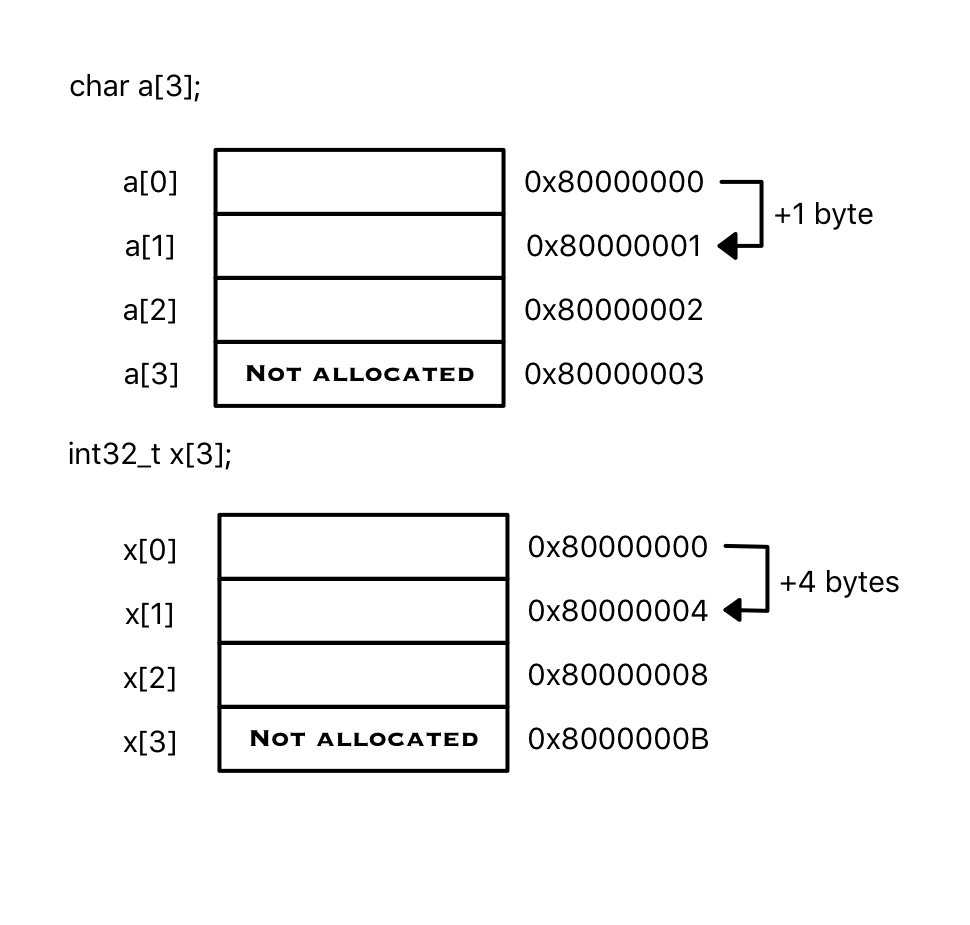
\includegraphics[width=0.6\textwidth]{array.jpg}}
\caption{One dimensional array}
\label{array}
\end{figure}

Figure \ref{array} shows two arrays with the same number of elements but different element sizes. The top array is an array of char's called \textit{a}. Each element of the array is offset by 1 byte taking up a total of four bytes. By comparison, the bottom array is an array of int's. Each element in the array is offset by 4 bytes and is taking up 16 (4x4) bytes. The elements in an \textit{int} array are separated by 4 bytes because i.e. \textit{sizeof(int32\_t)=4}		and for \textit{char}'s by 1 byte i.e. \textit{sizeof(char)=1}.

The sizing of the array looks to be off by one because an array starts at zero, meaning an array declared as \textit{x[4]} does not allocate space for \textit{x[4]} but for \textit{x[0]} to \textit{x[3]}. 

It is also important to realize that C does not check for out-of-bounds issues. This means it is relatively easy to make a mistake and access memory which has not been allocated, potentially causing instability or corruption in the system. The programmer has the responsibility to ensure this doesn't happen.

\begin{lstlisting}[language=C,showstringspaces=false,caption={File: array1d.c, one dimensional array},captionpos=b,label=array1d]

 1 #include <stdio.h>
 2 #include <stdlib.h>
 3 #include <time.h>
 4 
 5 int main (void)
 6 {
 7 char one[10];
 8 unsigned int x;
 9 
10 srand((unsigned int)time(NULL));
11 
12 printf ("\n* one dimensional array \n\n");
13 
14 // set up the one dimensional array
15 
16   for (x=0; x<=9; x++)
17     one[x] = rand() % 10;
18 
19 // printout the one dimensional array
20 
21 printf ("  ");
22   for (x=0; x<=9; x++)  
23     printf (" %d ",x);
24   printf ("\n\n");
25 printf ("0:");  
26   for (x=0; x<=9; x++)  
27     printf (" %d ",one[x]);    
28   printf ("\n\n");
29    
30 return 0;
31 }

INTERACTION

cc array1d.c
$ ./a.out

* 1 * one dimensional array 

   0  1  2  3  4  5  6  7  8  9 

0: 9  0  9  8  4  4  6  3  0  8 

$
\end{lstlisting}

Listing \ref{array1d} shows a one dimensional array of 10 elements i.e. 0 to 9 inclusive. The array \textit{one} is define on line:7. Each element of the array is assigned a random value from 0 to 9, see lines:16:17. Finally the array is printed out on lines:21-28.

\subsection{Two dimensional arrays}

\begin{lstlisting}[language=C,showstringspaces=false,caption={File: array2d.c, two dimensional array},captionpos=b,label=array2d]

 1 #include <stdio.h>
 2 #include <stdlib.h>
 3 #include <time.h>
 4 
 5 int main (void)
 6 {
 7 char two[10][10]; // two dimensional array
 8 unsigned int x,y;
 9 
10 srand((unsigned int)time(NULL));
11 
12 printf ("\n* two dimensional array\n\n");
13 
14 // set up the two dimensional array 
15 
16   for (x=0; x<=9; x++)
17     for (y=0; y<=9; y++)
18       two[x][y] = rand() % 10;
19    
20 // printout the two dimensional array
21 
22 printf ("  ");
23   for (x=0; x<=9; x++)  
24     printf (" %d ",x);
25   printf("\n\n");
26 
27   for (y=0; y<=9; y++)
28   {
29   printf ("%d:",y);
30     for (x=0; x<=9; x++)
31       printf (" %d ",two[x][y]);
32   printf ("\n");
33   }
34 printf ("\n");
35 
36 return 0;
37 }

INTERACTION

$ cc array2d.c
$ ./a.out

* 2 * two dimensional array

   0  1  2  3  4  5  6  7  8  9 

0: 2  8  7  0  1  5  1  8  8  8 
1: 3  3  6  8  3  6  1  1  0  6 
2: 3  7  6  9  8  0  0  0  6  9 
3: 1  4  4  8  5  3  7  3  6  1 
4: 8  8  1  8  2  0  5  0  4  5 
5: 2  4  9  2  8  9  8  5  1  9 
6: 9  6  2  1  1  8  0  5  5  0 
7: 9  3  7  6  1  9  9  9  2  8 
8: 1  4  4  1  2  1  6  3  5  8 
9: 8  7  0  4  5  8  2  9  8  3 

$
\end{lstlisting}


listing \ref{array2d} shows a two dimensional array of 10x10 elements. Line:7 declares the array. Lines:16-18 initializes the 2D array, again with a random number between 0 and 9. Once initialized the array is printed out, as carried out by the code on lines:22-34.

\subsection{Three dimensional arrays}


\begin{lstlisting}[language=C,showstringspaces=false,caption={File: array3d.c, three dimensional array},captionpos=b,label=array3d]

 1 #include <stdio.h>
 2 #include <stdlib.h>
 3 #include <time.h>
 4 
 5 int main (void)
 6 {
 7 char three[10][10][10]; // 3 dimensional array
 8 unsigned int x,y,z;
 9 
10 srand((unsigned int)time(NULL));
11 
12 printf ("\n* three dimensional array \n\n");
13 
14 // set up the three dimensional array
15 
16   for (x=0; x<=9; x++)
17     for (y=0; y<=9; y++)
18       for (z=0; z<=9; z++)
19         three[x][y][z] = rand() % 10;
20 
21 // printout the three dimensional array
22 
23   for (z=0; z<=9; z++)
24   {
25   printf ("\nz:%d\n",z);
26 
27   printf ("  ");
28     for (x=0; x<=9; x++)  
29       printf (" %d ",x);
30     printf("\n\n");
31 
32     for (y=0; y<=9; y++)
33     {
34     printf ("%d:",y);
35       for (x=0; x<=9; x++)
36         printf (" %d ",three[x][y][z]);
37     printf ("\n");
38     }
39   }
40 
41 return 0;
42 }

INTERACTION

$ cc array3d.c
$ ./a.out

* 3 * three dimensional array 

z:0
   0  1  2  3  4  5  6  7  8  9 

0: 6  8  9  8  7  3  1  7  5  8 
1: 2  3  9  7  5  2  8  2  8  7 
2: 9  4  4  6  2  7  8  3  0  3 
3: 9  5  9  8  8  4  8  5  5  6 
4: 1  2  5  4  7  2  4  9  3  1 
5: 2  0  3  9  2  7  7  4  1  2 
6: 4  8  8  2  6  3  1  7  7  9 
7: 2  2  6  6  2  8  9  6  0  7 
8: 1  0  9  0  8  3  5  3  3  3 
9: 2  5  5  8  3  6  7  0  1  8 

...

z:9
   0  1  2  3  4  5  6  7  8  9 

0: 1  5  2  8  5  3  8  7  4  8 
1: 2  6  3  8  3  0  3  2  2  9 
2: 7  3  8  8  0  1  8  0  9  4 
3: 9  7  9  8  0  9  2  5  6  6 
4: 9  4  2  6  5  5  6  7  3  5 
5: 9  3  2  5  8  3  0  5  8  9 
6: 1  1  6  5  0  5  4  1  3  4 
7: 8  5  4  6  7  9  4  7  7  9 
8: 2  7  5  0  6  6  1  4  4  8 
9: 4  9  5  5  0  7  5  9  7  1 

$

\end{lstlisting}

Listing \ref{array3d} shows a three dimensional array with 10x10x10 elements. Similar to listing \ref{array1d} and \ref{array2d} the array is created, initialized and displayed. The real difference being that a three dimensional array is more complicated to printout. 

For optimal performance, it is recommended that the code follow the layout of the target hardware cache. Hardware caches are designed with specific data lengths. The nearer any data format is to these lengths the more efficient and faster the throughput. This can have significant improvements on array manipulation performance since it can take advantage of the temporal and spacial characteristics of the target hardware. 

Particular performance cases may require some extra padded records. Enforcing data alignment with a specific cache architecture i.e. line length, can produce significant performance improvements although at the cost of increasing memory usage. This comes at the cost of increasing memory size. The inverse is to pack structures to maximize memory utilization. This may slow a program down due to the high frequency of cache misses. A general rule for optimal performance is to align data as much as possible with the cache architecture being used.

Arrays are used to create queues, circular buffers, stacks and strings in C.

\subsection{Passing arrays into functions}

Passing arrays into functions can be carried out using a number of different methods, as shown in listing \ref{arraypass}.

\begin{lstlisting}[language=C,showstringspaces=false,caption={File: arraypass.c},captionpos=b,label=arraypass]

 1 #include <stdio.h>
 2 #include <stdint.h>
 3 
 4 
 5 void print_out_1darray(char *a1,uint8_t size)
 6 {
 7   do
 8   {
 9   a1[size] = size;
10   printf("array[%d] = %d\n",size,a1[size]);
11   }
12   while (size--);
13 }
14 
15 void print_out_2darray(char a2[2][2])
16 {
17 uint8_t y=1,x;
18   do
19   {
20   x = 1;
21     do
22     {
23     a2[x][y] = x+y;
24     printf("array[%d,%d] = %d\n",x,y,a2[x][y]);
25     }
26     while (x--);
27   }
28   while (y--); 
29 }
30 
31 void print_out_3darray(char (*a3)[2][2])
32 {
33 uint8_t z=1,y,x;
34   do
35   {
36   y = 1;
37     do
38     {
39     x = 1;
40       do
41       {
42       a3[x][y][z] = x+y+z;
43       printf("array[%d,%d,%d] = %d\n",x,y,z,a3[x][y][z]);
44       }
45       while (x--);
46     }
47     while (y--);
48   }
49   while (z--);
50 }
51    
52 int main(void)
53 {
54 char _a1[2],_a2[2][2],_a3[2][2][2];
55 
56 print_out_1darray(_a1,1);
57 print_out_2darray(_a2);
58 print_out_3darray(_a3);
59 
60 return 0;
61 }

INTERACTION

$ cc arraypass.c
$ ./a.out
array[1] = 1
array[0] = 0
array[1,1] = 2
array[0,1] = 1
array[1,0] = 1
array[0,0] = 0
array[1,1,1] = 3
array[0,1,1] = 2
array[1,0,1] = 2
array[0,0,1] = 1
array[1,1,0] = 2
array[0,1,0] = 1
array[1,0,0] = 1
array[0,0,0] = 0
$
\end{lstlisting}

Listing \ref{arraypass} shows a method to pass a single dimensional array, a two dimensional array and a three dimensional array. The first example, \textit{print\_out\_1darray(...)} shows a one dimensional array being passed in, as shown on lines:5-13. The array is passed as a pointer plus an argument defining the size of the array. 

The second example on lines:15-29 \textit{print\_out\_2darray(...)}, shows a two dimensional array with a fixed size [2][2]. 

Finally the third example on lines:31-50 \textit{print\_out\_3darray(...)}, shows a three dimensional array being passed as a pointer to a fixed two dimensional array [2][2]. Essentially passing an array into a function is basically passing the address of the beginning of the array. 

